\label{chap:machine_learning}
\section{Preparazione dei dati per il task di ML}

\subsection{Estrazione dei dati}

Procediamo con l'estrazione di un dataset tramite la query SQL che
interroga le tabelle \texttt{hj} e \texttt{htjob}. Ricordando che:
\begin{itemize}
    \item La tabella \texttt{hj} contiene lo stato dei job, rappresentato da
        serie storiche di misurazioni (come \texttt{runtime}, \texttt{ram},
        \texttt{swap}, \texttt{disk}, ecc.),
        durante la loro esecuzione.
    \item La tabella \texttt{htjob} fornisce informazioni sull'esito dei job,
        ovvero se sono falliti o meno.
\end{itemize}

La query esegue le seguenti operazioni:
\begin{itemize}
    \item Seleziona i job che hanno iniziato e finito la loro esecuzione nel
        periodo temporale specificato.
    \item Esegue un JOIN delle tabelle utilizzando l'identificativo univoco di
        ciascun job (\textit{jobid.idx\_submitnode}) e il timestamp. Questo
        timestamp sfrutta l'indice presente nella tabella
        \texttt{hj} per gestire in maniera efficiente le grandi dimensioni di
        questa tabella\footnote{la logica dietro questo consiste
            nel selezionare un job da \texttt{htjob} e successivamente
            cercarlo in \texttt{hj} limitando la ricerca ai record che
            rientrano nel periodo in cui \texttt{hj.ts} è compreso tra
            \texttt{htjob.starttimeepoch} e \texttt{htjob.eventtimeepoch}.
            Questo permette di restringere notevolmente la ricerca nella
            tabella \texttt{hj} per ogni job selezionato da \texttt{htjob} ed
        evitare di scansionare l'intera tabella.}. Poiché la tabella \texttt{hj} contiene più record per
        ogni job, la query li raggruppa per job. In seguito, mediante l'uso
        dell'operatore \verb|ARRAY_AGG|, le serie storiche vengono trasformate
        in liste di valori.
    \item Filtra i job con un tempo di esecuzione superiore a un'ora
        (\verb|runtime > 3600|), in quanto i job più brevi sono considerati
        irrilevanti per lo scopo dello studio.
\end{itemize}

Il risultato di questa query è un dataset come mostrato nella
figura~\ref{fig:dataset_from_join_hj_htjob}, dove ogni riga rappresenta un job
e le colonne includono: 

\begin{itemize}
    \item \texttt{job}: identificativo univoco per ogni job.
    \item \texttt{queue}: gruppo di appartenenza dell'utente che ha sottomesso
        il job.
    \item \texttt{fail}: una variabile booleana che indica se il job è fallito.
    \item \texttt{mint} e \texttt{maxt}: il tempo minimo e massimo di
        esecuzione del job.
    \item \texttt{t}, \texttt{ram}, \texttt{swap}, \texttt{disk}: liste di
        valori che rappresentano le serie storiche di misurazioni.
\end{itemize}



%\begin{lstlisting}[language=SQL, caption={Esempio di codice SQL},
%    label={lst:my_sql_code}]
%WITH A AS (
%    SELECT 
%        CONCAT(j.jobid, '.', j.idx, '_', jd.fromhost) AS job,
%        jd.queue,
%        (jd.jobstatus != 4 OR jd.exitstatus != 0)::int AS fail,
%        MIN(j.ts) AS mint,
%        MAX(j.ts) AS maxt,
%        ARRAY_AGG(j.rt ORDER BY j.rt ASC) AS t,
%        ARRAY_AGG(j.rss ORDER BY j.rt ASC) AS ram,
%        ARRAY_AGG(j.swp ORDER BY j.rt ASC) AS swap,
%        ARRAY_AGG(j.disk ORDER BY j.rt ASC) AS disk
%    FROM (
%        SELECT ts, jobid, idx, queue, rt, rss, swp, disk
%        FROM hj
%        WHERE ts BETWEEN to_unixtime('2023-03-13') - 3600 AND
%        to_unixtime('2023-04-01') - 3600
%    ) j 
%    INNER JOIN htjob_recent jd ON
%        j.queue = jd.queue AND
%        j.jobid = jd.jobid AND
%        j.idx = jd.idx AND
%        j.ts BETWEEN jd.starttimeepoch AND jd.eventtimeepoch
%    WHERE
%        jd.eventtimeepoch BETWEEN to_unixtime('2023-03-13') AND
%        to_unixtime('2023-04-01') AND
%        jd.runtime >= 3600
%    GROUP BY job, jd.queue, fail
%    ORDER BY mint
%)
%SELECT 
%    job,
%    queue,
%    fail,
%    mint,
%    maxt,
%    t,
%    ram,
%    swap,
%    disk
%FROM A
%WHERE t[1] <= 180
%\end{lstlisting}

\begin{figure}[!ht]
    \centering
    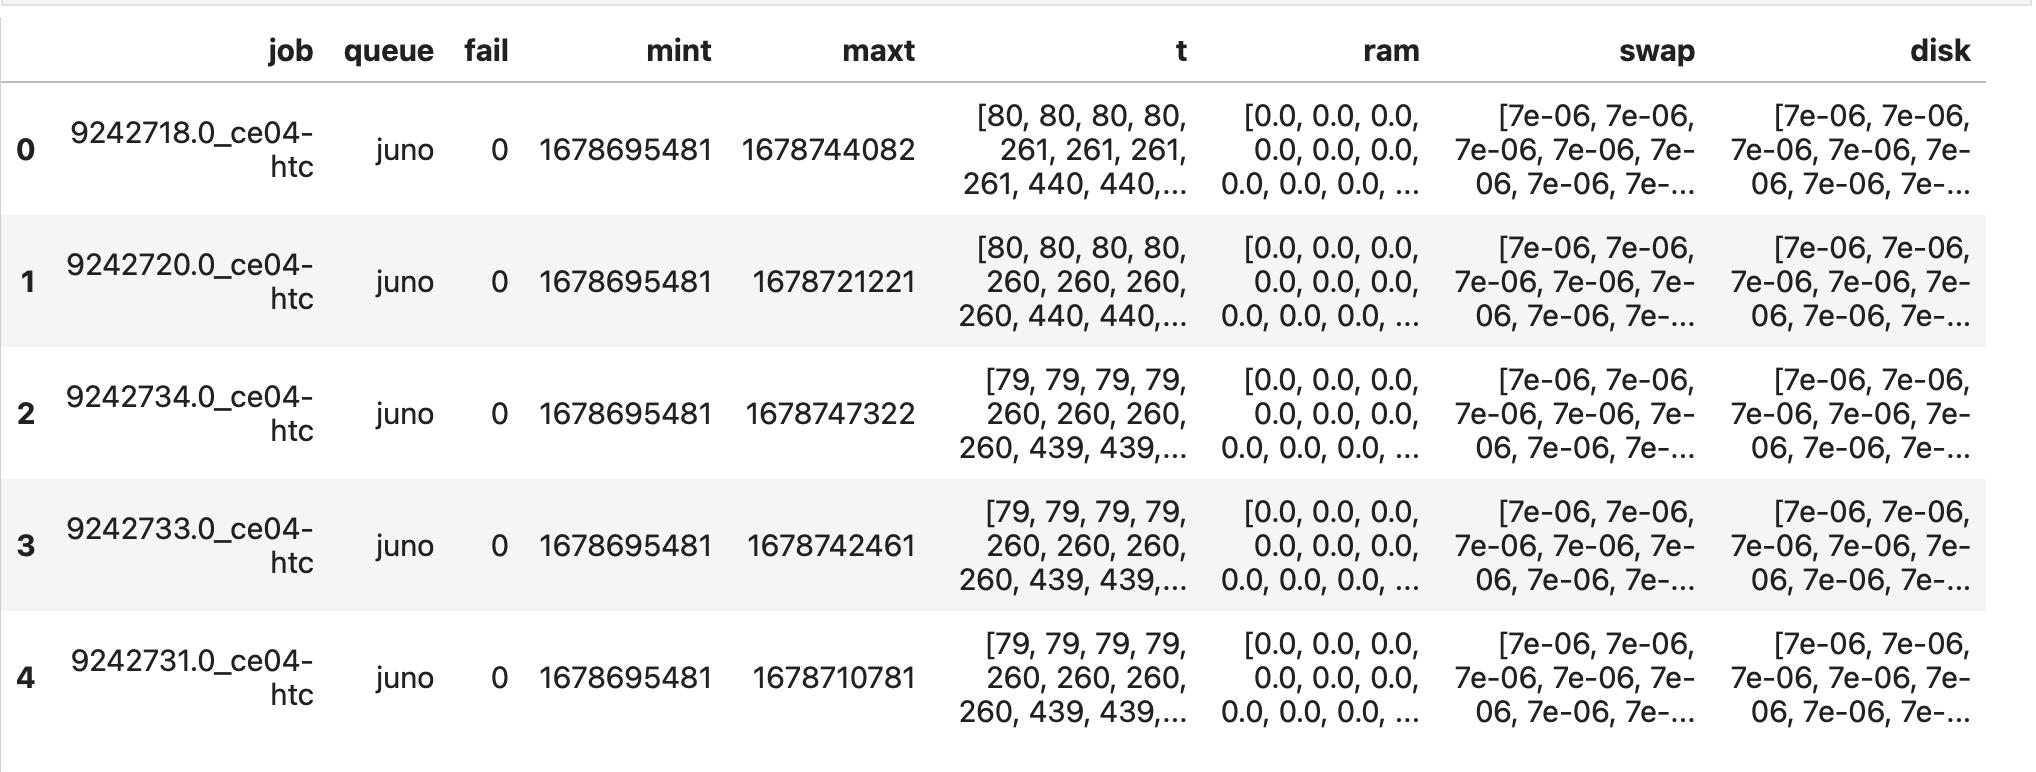
\includegraphics[width=0.95\textwidth]{dataset}
    \caption{Le prime cinque righe del dataset}
    \label{fig:dataset_from_join_hj_htjob}
\end{figure}


\subsection{Trasformazione delle serie storiche multivariate multiple}

% 

% dobbiamo convertire le serie storiche in un tipo di dati strutturato,
% tabellare, utilizzabile dai modelli di Machine Learning

% padding e truncate delle serie storiche 

% avg pooling

% tabular transformation

% tensor transformation

\subsection{Creazione delle feature}
\begin{figure}[!ht]
    \centering
    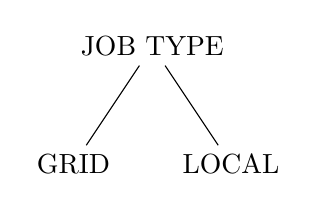
\begin{tikzpicture}[sibling distance=2cm]
        \node {JOB TYPE}
            child {node {GRID}}
            child {node {LOCAL}};
    \end{tikzpicture}
    \hspace{2cm}
    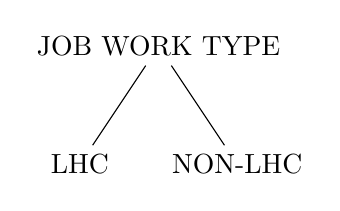
\begin{tikzpicture}[sibling distance=2cm]
        \node {JOB WORK TYPE}
        child {node {LHC}}
        child {node {NON-LHC}};
    \end{tikzpicture}
\end{figure}

% jobid e idx

% jobid e idx sono creati dal Submit Node al "concepimento" del job (es.
% 'sn-01', 'ce03-htc', ...). I S.N. sono indipendenti tra loro per cui in linea
% di principio possono esistere due job diversi con (jobid,idx) uguale (in tal
% caso vengono da S.N. diversi)%

% job work type

% job type

% one hot encoding 

% non verranno considerati i jobs con runtime <
% 1h, poichè non rilevanti per il sistema.

\subsection{Etichettatura dei dati}

% Una possibile strategia:
% - usando htjob si trovano i job eliminati per "toomuchtime": sono quelli con
%   jobstatus = 3 e runtime ~=7gg (non c'è valore esatto!)
% - a questo punto possiamo possiamo impostare un supervised learning
%   guardando su hj come hanno "vissuto" quei job.

\subsection{Tecniche di bilanciamento dei dati}

% undersample

% oversample

% class weighting in loss function

% metriche
\section{Selezioni dei modelli}
\subsection{Modelli supervisionati}
\subsection{Modelli non supervisionati}
\section{Valutazione delle performance}
\subsection{Metriche di valutazione}
\subsection{Convalida incrociata}
